\documentclass{article}

\usepackage{amsmath}
\usepackage{graphicx}

\newcommand{\PosC}{\mathrm{Pos}}
\newcommand{\NegC}{\mathrm{Neg}}

\begin{document}

\section{Method}

\subsection{Document Representation}

We tried four different document representations: as bags of words for the multinomial model; as sets of words for the Bernoulli model; and both of these after applying the Porter Stemming Algorithm.

\subsection{Model and Training}

We use a na\"ive Bayes classifier: for a class \(c \in \{\PosC, \NegC\}\) and document \(d\) consisting of words \(w_{d,1},\dotsc,w_{d,m_d}\) (where each word occurs at most once in the Bernoulli version),
\[\Pr(c|d)=\frac{\Pr(d|c)\Pr(c)}{\Pr(d)}\]
where
\[\Pr(d|c)=\sum_{i=1}^{m_d}\Pr(w_i|c)\ldotp\]
and our training procedure produces
\[\Pr(w|c)=\frac{n_{w,c}+\alpha}{\sum_{w'}(n_{w',c}+\alpha)}\ldotp\]
We try different values for \(\alpha\) as explained in Section~\ref{sec:EvalAndTuning}.

\subsection{Evaluation and Parameter Tuning}
\label{sec:EvalAndTuning}

To avoid confusion, we will refer to positive reviews as ``favorable'' and negative reviews as ``disfavorable'' in this section.  We chose evaluate the model's performance on a testing set using the \(F_1\) score.  The \(F_1\) score is defined as:
\[
  F_1=
  \frac
      {2\cdot\#\text{true positive}}
      {2\cdot\#\text{true positive}+\#\text{false negative}+\#\text{false positive}}
  \ldotp
\]
We had some difficulty interpreting this in the context of a classification task.
We decided that the score makes sense when focusing on a particular label.
For example, if we are interested in the model's performance with the label ``favorable'', then we count test results as follows.

\begin{tabular}{c|c|c}
  true class & model classification & interpretation for ``favorable'' \\
  \hline
  favorable & favorable & true positive \\
  favorable & disfavorable & false negative \\
  disfavorable & favorable & false positive \\
  disfavorable & disfavorable & true negative \\
\end{tabular}

We define the resulting score to be \(F_1(\PosC)\).
We define \(F_1(\NegC)\) the same way but with the roles of ``favorable'' and ``disfavorable'' reversed, and score documents as
\[\text{document score}=\tfrac12 (F_1(\PosC) + F_1(\NegC)) \ldotp\]
The score of the model is the sum of the document scores.

We had three parameters to tune: multinomial or Bernoulli; whether to stem words; and the smoothing parameter \(\alpha\).  We tried all combinations of the first two parameters, with \(\alpha\) varying between \(0.1\) and \(30\) with a ratio of \(\sqrt{2}\) between successive \(\alpha\)-values (\(0.1, 0.1\sqrt{2}, 0.2, 0.2\sqrt{2}, \dotsc\)).  Using a geometric series allowed us to try many ranges of size for the \(\alpha\) parameter; once we identified the range with the best performance, we did a second pass with a finer range of \(\alpha\)-values as explained in Section~\ref{sec:Results}.

We used 10-fold cross-validation to evaluate the performance of our algorithm.  We chose a random order for the documents once, and for each parameter setting, we evaluated the model ten times (using successive slices as the held-out test set) and recorded the average score of the model on those ten sets.


\section{Experiments}
\label{sec:Results}

We implemented our Na\"{i}ve Bayes sentiment classifier in Scala 2.9.1 and tested the classifier on the polarity movie review dataset \cite{polarity-dataset}. The dataset contains 1000  

\begin{figure}
  \centering
  \caption{F1 measures for various combinations of parameters.}
  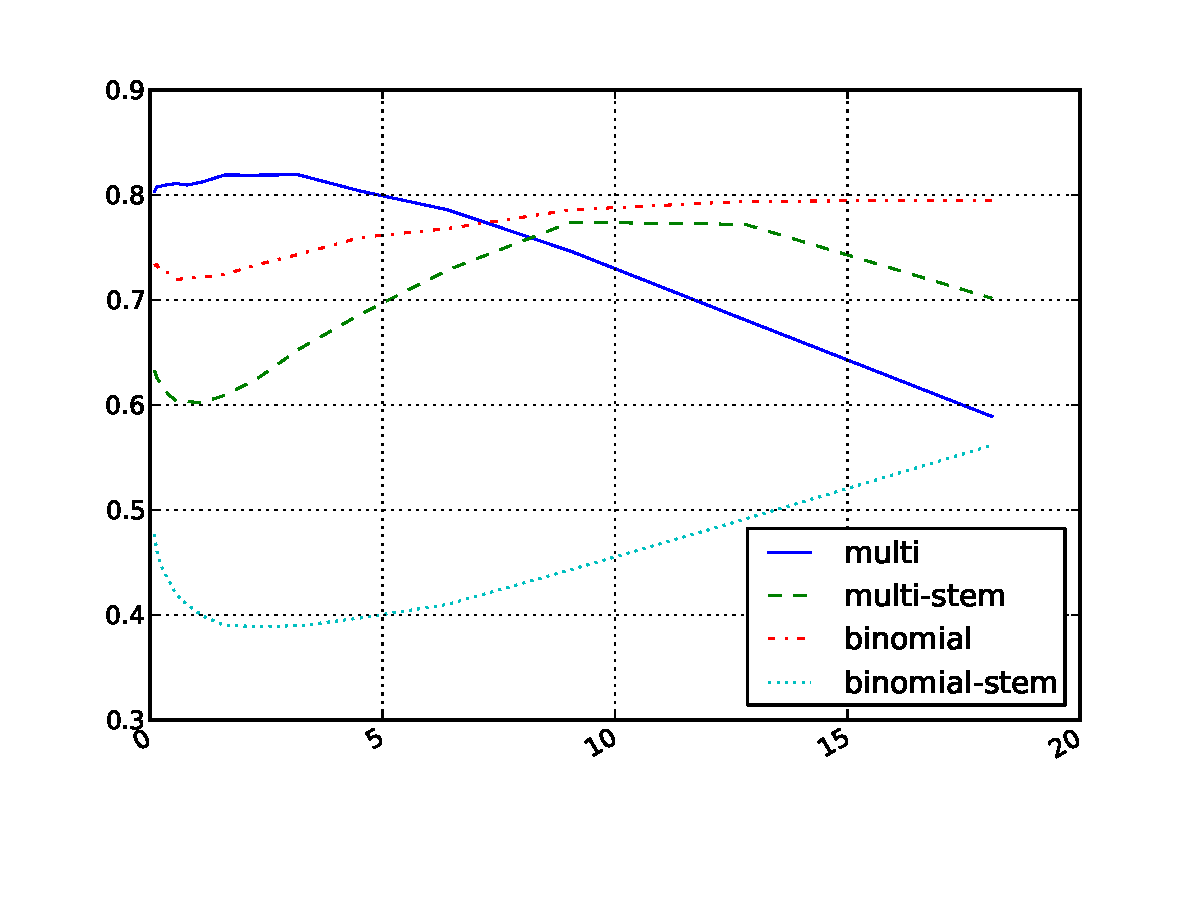
\includegraphics[width=\textwidth]{graphs/all-combo.pdf}
\end{figure}




\subsection{Stemming}

%Stemming is the process of reducing inflected and derived words to their stem \cite{porter-stemmer}. Stemming incidentally reduces the number of features used in the classifier. For example, using the Porter Stemmer \cite{porter-stemmer}, both ``apply'' and ``applying'' become the same stem ``appli''.

We observed that stemming the words had a negative impact on the F1 score, while using more computational resources. We speculate that the choices of variations of words indeed carry connotations on sentiments. This observation is consistent with findings from previous works \cite{stanford-tutorial, sentiment-twitter}.


\subsection{Binomial vs Multinomial}


\subsection{Smoothing}

\begin{figure}
  \centering
  \caption{Tuning smoothing factor alpha.}
  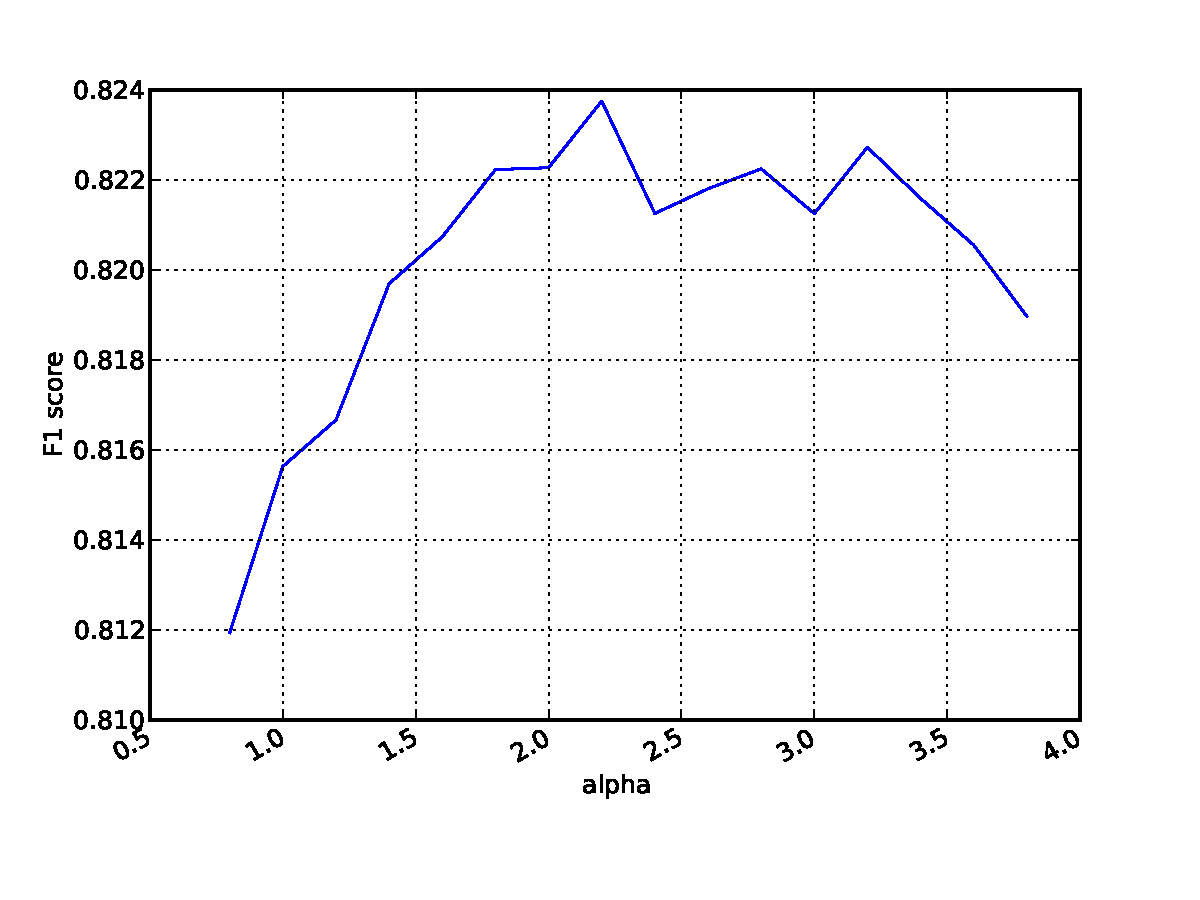
\includegraphics[width=\textwidth]{graphs/alpha.pdf}
\end{figure}


\subsection{Top Term Weights}

% Program output:
%(false,false,2.2,0.822)
%Pos: List((shrek,3.230), (mulan,3.138), (flynt,2.9035111177554587), (gattaca,2.8346396128564333), (ordell,2.759), (truman's,2.6187512324233975), (lebowski,2.6168669281160994), (guido,2.588), (leila,2.55661945131639), (sweetback,2.490))
%Neg: List((nbsp,-3.4045562750852802), (seagal,-3.1096499422617025), (brenner,-2.747), (sphere,-2.572643333537556), (schumacher,-2.556), (stigmata,-2.493), (1900,-2.451), (pokemon,-2.406976211648738), (bye,-2.406976211648738), (jawbreaker,-2.404))
%Pos (mf): List((,,6988.590), (the,5680.522), (and,5062.829), (is,3480.295), (of,3031.905), (his,2302.1047630517264), (as,2103.495762997044), (he,1394.452), (in,1206.934), (a,976.3928793058776))
%Neg (mf): List((.,-3176.335), (",-2935.369), (i,-1874.9698007890427), (movie,-1832.499865514896), (?,-1631.999), (bad,-1574.092), (this,-1474.2238454822032), (have,-1308.290), (!,-974.078), (no,-939.664))


This is for our best set of model parameters: multinomial model; no stemming; \(\alpha=2.2\).

\begin{figure}
\begin{tabular}{c|c}
    \multicolumn{2}{c}{Tokens most likely to be positive} \\
    token & \(log(p_+ / p_-)\) \\
    \hline
    shrek & 3.230 \\
    mulan & 3.138 \\
    flynt & 2.904 \\
    gattaca & 2.835 \\
    ordell & 2.759 \\
    truman's & 2.619 \\
    lebowski & 2.617 \\
    guido & 2.588 \\
    leila & 2.557 \\
    sweetback & 2.490
\end{tabular}
\begin{tabular}{c|c}
    \multicolumn{2}{c}{Tokens most likely to be negative} \\
    token & \(log(p_+ / p_-)\) \\
    \hline
    nbsp & -3.405 \\
    seagal & -3.110 \\
    brenner & -2.747 \\
    sphere & -2.573 \\
    schumacher & -2.556 \\
    stigmata & -2.493 \\
    1900 & -2.451 \\
    pokemon & -2.407 \\
    bye & -2.407 \\
    jawbreaker & -2.404
\end{tabular}
\caption{Highest-weighted tokens.}
\end{figure}

\begin{figure}
\begin{tabular}{c|c}
    \multicolumn{2}{c}{Most influential positive tokens} \\
    token & \((\# \mathrm{occurrences}) \cdot \log(p_+ / p_-)\) \\
    \hline
     , & 6989 \\
    the & 5681 \\
    and & 5063 \\
    is & 3480 \\
    of & 3032 \\
    his & 2302 \\
    as & 2103 \\
    he & 1394 \\
    in & 1207 \\
    a & 976.4
\end{tabular}
\begin{tabular}{c|c}
    \multicolumn{2}{c}{Most influential negative tokens} \\
    token & \((\# \mathrm{occurrences}) \cdot \log(p_+ / p_-)\) \\
    \hline
    . & -3176 \\
    " & -2935 \\
    i & -1875 \\
    movie & -1832 \\
    ? & -1632 \\
    bad & -1574 \\
    this & -1474 \\
    have & -1308 \\
    ! & -974.1 \\
    no & -939.7
\end{tabular}
\caption{Tokens with highest \((\mathrm{weight} \cdot \# \mathrm{occurrences})\).}
\end{figure}


\subsection{Parallelization}



\bibliographystyle{plain}
\bibliography{report}

\end{document}
